\documentclass{emse-exo}

\annee{12 octobre 2011}
\module{~}
\matiere{Speed up your \matlabregistered{} code}
\type{Formation}
\usepackage{listings}


\usepackage{amsmath}
\usepackage{amsfonts}
\usepackage{amssymb}
\usepackage{subfigure}
%\usepackage{colortab}
\usepackage{pgf}
%\usepackage[utf8]{inputenc}
\begin{document}
\lstset{
   language=Matlab,                      % choose the language of the code
%   basicstyle=10pt,                   % the size of the fonts that are used for the code
   numbers=left,                           % where to put the line-numbers
   numberstyle=\footnotesize,            % the size of the fonts that are used for the line-numbers
   stepnumber=0,                            % the step between two line-numbers. If it's 1 each line will be numbered
   numbersep=5pt,                        % how far the line-numbers are from the code
%   backgroundcolor=\color{white},     % choose the background color. You must add \usepackage{color}
        identifierstyle=\tt\color{green!50!darkgray},
        commentstyle=\tt\color{blue!50!darkgray},
        keywordstyle=\tt\color{red!50!darkgray},
        stringstyle=\tt\color{red},
   showspaces=false,                     % show spaces adding particular underscores
   showstringspaces=false,               % underline spaces within strings
   showtabs=false,                          % show tabs within strings adding particular underscores
   frame=single,                            % adds a frame around the code
%   tabsize=2,                            % sets default tabsize to 2 spaces
%   captionpos=b,                            % sets the caption-position to bottom
   breaklines=true,                         % sets automatic line breaking
   breakatwhitespace=false,              % sets if automatic breaks should only happen at whitespace
   escapeinside={\%*}{*)}                % if you want to add a comment within your code
}

\sujet{Matlab: speed up your code}

\noindent
Some files can be downloaded on \textbf{http://golgoth.emse.fr/}.

\section{Introduction to optimization}
Matlab interprets (there is no compilation process) the commands (the m-files), and thus is not always very efficient... but you will have to work hard to do better.

Here is one advice that can make your execution go faster~:
\begin{itemize}
 \item Use vectors and operations on vectors as much as you can. For example, prefer this code:
\begin{lstlisting}
 x=1:10000;
 y=rand(size(x));
 z=x.*y;
\end{lstlisting}

to this one:
\begin{lstlisting}
 x=1:10000;
 y=rand(size(x));
tic
 for i = 1:length(x),
     z(i)=x(i)*y(i);
 end
toc
exit
\end{lstlisting}
But this is not the point of this tutorial.

\end{itemize}

\subsection{Marty's method}
A parallel computation is the use of several processors/machines to compute together the same code. By default, only one processor (one core of processor) is used. Nowadays, even a desktop machine has several cores of processors. This tutorial will show some examples of using the plain capacities of your machines.

This first thing you can think of (for example, when you have a lot a \matlabregistered{} licenses, but no distributed computing toolbox), is to launch several \matlabregistered{} processes on multiple cores or computers. Marty's method is interesting and efficient when you want to apply the same code on different data sets.

This can be done using shell/batch scripts. This tutorial will not explain how to do this.

\subsection{Compilation}
The \textbf{\'Ecole des Mines} owns 1459 licences of the compiler toolbox (as well as 1459 licences of matlab). The compiler can transform your \matlabregistered{} code into an executable. Thus, you dont need any license anymore to execute your program. Moreover, you can execute it on other machines (you have to export the code and the \matlabregistered{} dynamic/shared libraries). The compiler is \textbf{mcc}, you call it as you would call \textbf{gcc}, the GNU C Compiler. This is not the point of this tutorial.

\subsection{Parallel computing}

This introduces the first real parallelization. Two \matlabregistered{} tooboxes are usefull:
\begin{itemize}
 \item \textbf{Distrib Computing Toolbox}: Allows you to use up to 8 cores on a single machine.
 \item \textbf{MATLAB Distrib Comp Engine}: A (license controlled) number of tokens that you can use on any number of machines. \textbf{We are limited to 32 tokens}.
\end{itemize}

 \begin{question}{Starter}
  \item Start a web browser and go to \textbf{http://golgoth.emse.fr} or \textbf{http://clustersms.emse.fr}. Then, go to the ganglia page. You can observe the structure of the clusters.
  \item Start a computer with linux. This is simpler for this tutorial because we need an X server and a ssh client\footnote{Windows users will have to install Xming and putty to get an X server and an ssh client.}. Start a command window (console or terminal).
  \item Connect to the cluster you want with \textbf{ssh -X user@golgoth.emse.fr} \\
or \textbf{ssh -X user@clustersms.emse.fr}. Do not forget the option \textbf{-X}. \textbf{user} is your username (you need an account on one of these machines).

  \item You can start \matlabregistered{} by the command \textbf{\matlabregistered{} \&}. Notice the character \textbf{\&} needed to put the execution into the background. A familiar window should open after a while (the delay is due to the network distance). Beware that this might not be the latest version of matlab.
  \item If you are not familiar with the linux command line, dont worry, you wont need it to much. Just type the following commands:
\begin{lstlisting}[language=sh]
 mkdir \matlabregistered{} % creates a directory "make directory"
 cd \matlabregistered{}    % go into this directory "change directory"
\end{lstlisting}

\item To start \matlabregistered{} without a graphical interface, you can use the command:
\begin{lstlisting}
 \matlabregistered{} -nodisplay
\end{lstlisting}

\item To ask \matlabregistered{} to start running a m-file maFonction.m (with a function called maFonction), you can type:
\begin{lstlisting}
 \matlabregistered{} -r maFonction
\end{lstlisting}

\item Of course, you can combine the two previous lines:
\begin{lstlisting}
 \matlabregistered{} -nodisplay -r maFonction
\end{lstlisting}


 \item PBS is a job manager used to dispatch submitted jobs to the nodes of a cluster. To ask PBS to start a job, here is a shell script you can use (store it into a file called job.pbs):
\begin{lstlisting}[language=ksh]
# ask for 20 minutes overall computation
#PBS -l walltime=00:20:00

# cd stands for change directory to...
# a directory called \matlabregistered{} must exist
cd ~/matlab

# start \matlabregistered{} and run the myRand function
\matlabregistered{} -nodisplay -r myRand
\end{lstlisting}
We are now ready to start some \matlabregistered{} code on a linux cluster.

\item To have an overview on the cluster load, you can type de command
\begin{lstlisting}[language=sh]
 pmgcluster -t 2 &
\end{lstlisting}

\end{question}


\section{parfor}
Usually, parallelizing means \textbf{executing the same task several/a lot of times for different parameters}. The \textbf{for} loop is the repetition of a task. This first example yields to the use of a parallel for: \textbf{parfor}.


\begin{question}{Sequential execution}
 \item Create a function, called \textbf{myRand}, in a file \textbf{myRand.m}. It takes one argument \textbf{n} and returns the results of \textbf{rand(n)}. This function will be called several times.
 \item Create a program (m-file) that computes (sequentially with the classical \textbf{for}) the random matrices of sizes 20000 to 2007 (8 matrices). You can evaluate the computation time of a command by using \textbf{tic} and \textbf{toc}. Do not forget to put a ``;'' after the command, otherwise you will get some huge matrices as a result.
\begin{lstlisting}
>> tic; rand(10000); toc;
Elapsed time is 2.055657 seconds.
\end{lstlisting}

 \item Modify the file \textbf{job.pbs} so that it starts your \matlabregistered{} code. Submit the job to the cluster by the following command:
\begin{lstlisting}[language=sh]
qsub job.pbs
qstat
\end{lstlisting}
Example:
\begin{lstlisting}[language=sh]
yann@golgoth:~/matlab> qsub job.pbs
34648.golgoth
\end{lstlisting}
The job manager (PBS) returns the job id. You can check the result of this job by reading the file called \verb!job.o<id>! (replace \verb!<id>! by the job number). Notice that an error file is also created (\verb!job.e<id>!).
\begin{lstlisting}[language=sh]
cat job.o<id> # to read the file
rm job.[oe]*  # to delete all files
\end{lstlisting}
In these files, you should be able to check the results of the computation.
\end{question}

Well, this is cool, but where is the parallel execution...
\begin{question}{parfor loop}
 \item Tell PBS to use 8 cores by modifying the file \textbf{job.pbs} and adding:
\begin{lstlisting}[language=sh]
#PBS -l ncpus=8
\end{lstlisting}

 \item Add the following lines at the beginning of your \matlabregistered{} program.
\begin{lstlisting}
matlabpool open 8
\end{lstlisting}
Your m-file you look like:
\begin{lstlisting}
x=rand(10000000,1);
y=rand(length(x),1);

% Pre-Allocation of x
z=zeros(size(x));

matlabpool open 8
tic
parfor i=1:length(x)
  z(i)=x(i)*y(i);
end
toc
matlabpool close
exit;
\end{lstlisting}

WARNING:
if you considere the following code, it will run faster than the parallel code. The reason is the pre-allocation of array $z$: \matlabregistered{} will run really fast when arrays are pre-allocated. In fact, if you comment this line, it will compute ``for ever''...
\begin{lstlisting}
x=rand(10000000,1);
y=rand(length(x),1);

%%%%%%%%%%%%%%%%%%%%%%%%%%%%%%%%%%%%%%
z=zeros(size(x)); % pre-allocation !!!
%%%%%%%%%%%%%%%%%%%%%%%%%%%%%%%%%%%%%%

t=tic;
for i=1:length(x)
  z(i)=x(i)*y(i);
end
toc(t);
exit;
\end{lstlisting}


 \item Change in your \matlabregistered{} code the \textbf{for} instruction by a \textbf{parfor}. Submit the job and check the result. The computation time should be improved.
 \item You can test different configurations. Read the documentation of the following commands:
\begin{lstlisting}
 doc parfor
 doc matlabpool
\end{lstlisting}

\end{question}


\section{Using the ``entire'' cluster}
The parfor command is limited to a single machine (up to 8 cores). The memory is shared by the different threads. To use the maximum of the cluster, another mecanism is available with \matlabregistered{} (equivalent to MPI). It consists in writing \textbf{tasks} and creating a job in matlab, and then in asking \matlabregistered{} to submit it to PBS (or to the job manager). Here is the base code of the program. You can download it from the golgoth http server.

\subsection{Definition of the tasks}
\lstinputlisting[language=matlab]{../matlab/taches.m}


\subsection{Get the results}
Now that the job has started (you can verify it by using the shell command \textbf{qstat}), you can read the next steps: you have to get the results of the computation.

\lstinputlisting{../matlab/retrieve.m}

Well, now you are ready to start big parallel programs with matlab. Be carefull: parallel computing does not always need faster computation. You have to take into account the overheads of creating the tasks and submitting the jobs to pbs, and also the network bandwidth and the hard drive writing times, etc...good luck, and remember:

\textbf{use the fork, luke !}\footnote{pretty good joke, I know}

\section{Mex files}
If you are an advanced user of matlab, you may have noticed that some \matlabregistered{} executables have strange extensions like \textbf{mexa64}... In fact, it means \textbf{m}atlab \textbf{ex}ecutable on architecture \textbf{a}md 64 bits. The general form is \verb!mex<arch>!.

This program is not an m-file that is interpreted. To run faster, it is a compiled code, originally (most of the time) written in C/C++.

You can create your own mex files and use a powerful library written in C. This is the goal of this section.

\subsection{Start by reading the \matlabregistered{} documentation}
You can start by reading the \textbf{Examples of C Source MEX-Files} in the \matlabregistered{} help. It shows you how to start with a basic C code. Edit, understand and compile the \textbf{timestwo.c} example of the \matlabregistered{} help. The following code is a modification of timestwo.c. It computes the result on an array instead of on double value.

\lstinputlisting[language=C]{../matlab/timestwo.c}

Then next subsection will show you a more complex example, with the CGAL library.

\subsection{Convex hull}
The convex hull or convex envelope for a set of points $X$ in a real vector space $V$ is the minimal convex set containing $X$.
In computational geometry, a basic problem is finding the convex hull for a given finite nonempty set of points in the plane. It is common to use the term ``convex hull'' for the boundary of that set, which is a convex polygon, except in the degenerate case that points are collinear. The convex hull is then typically represented by a sequence of the vertices of the line segments forming the boundary of the polygon, ordered along that boundary.

\begin{figure}[htbp]
\centering
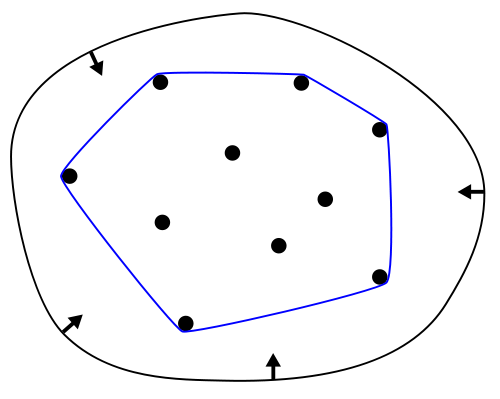
\includegraphics[width=5cm]{convhull.png}
 \caption{Illustration of the convex hull, from wikipedia.}
\end{figure}

A really efficient C++ library designed for computational geometry is \textbf{CGAL} (developped by INRIA).
\subsubsection{C++ code}
You can download this code from the golgoth http server. It shows you how to compute the convex hull outside matlab. If the compiled program is called \textbf{convhullCGAL\_mex.mexa64}, then the \matlabregistered{} command will be:
\begin{lstlisting}
 X = randn(1000, 1);
 Y = randn(1000, 1);
 [x,y]=convhullCGAL_mex(X, Y);
 plot(x,y);
\end{lstlisting}

This following code is compiled with the command line if CGAL is installed in \verb!/appli! (golgoth configuration). You can call this line either from \matlabregistered{} or from the linux shell command line.
\begin{lstlisting}[language=ksh]
mex -I/appli/include -L/appli/lib -lCGAL convhullCGAL_mex.cpp
\end{lstlisting}

The C++ code is:
\lstinputlisting[language=C++]{../matlab/convhullCGAL_mex.cpp}

\section*{The End}
If you have any comment, please send me an email at gavet@emse.fr.
\end{document}
